\documentclass[spanish]{beamer}
%
% Choose how your presentation looks.
%
% For more themes, color themes and font themes, see:
% http://deic.uab.es/~iblanes/beamer_gallery/index_by_theme.html
%
\mode<presentation>
{
  \usetheme{Ilmenau}      % or try Darmstadt, Madrid, Warsaw, ...
  \usecolortheme{lily} % or try albatross, beaver, crane, ...
  %usecolortheme{default} % or try albatross, beaver, crane, ...
  %\usefonttheme{default}  % or try serif, structurebold, ...
  \setbeamertemplate{navigation symbols}{}
  \setbeamertemplate{caption}[numbered]
  \setbeamertemplate{section in toc}{\inserttocsectionnumber.~\inserttocsection}
} 

\usepackage[spanish]{babel}
\usepackage[utf8x]{inputenc}

%\AtBeginSection{\frame{\sectionpage}}

\title[bioGUNE || Fabricación GUVs]{Colaboración bioGUNE:\\ Fabricación GUVs}
\author{Unai Eletxigerra}
\institute{IK4-Tekniker}
\date{10.06.2017}

\begin{document}

\begin{frame}
  \titlepage
\end{frame}

% Uncomment these lines for an automatically generated outline.
\begin{frame}{Índice}
 \tableofcontents
\end{frame}

\section{Objetivo}

\begin{frame}{Objetivo}
 \emph{Célula Artificial} mediante modelos simplificados: Membrana celular\\
  \vfill
  \centering
  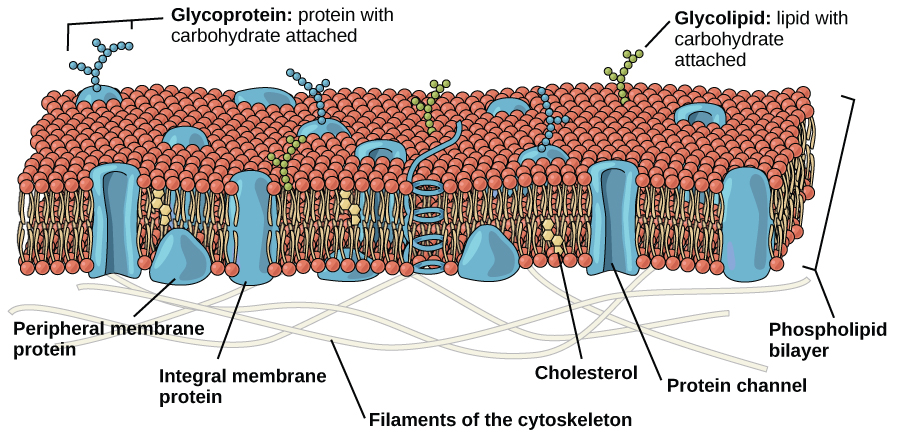
\includegraphics[width=0.7\textwidth]{img/membrane}
  \vfill
  \raggedright
  Se requieren métodos de fabricación fiables y reproducibles
\end{frame}

\section{Vesículas}

\begin{frame}{Liposomas}
  Liposomas (vesículas): Solución acuosa delimitada por una bicapa.
  \vfill
  \centering
  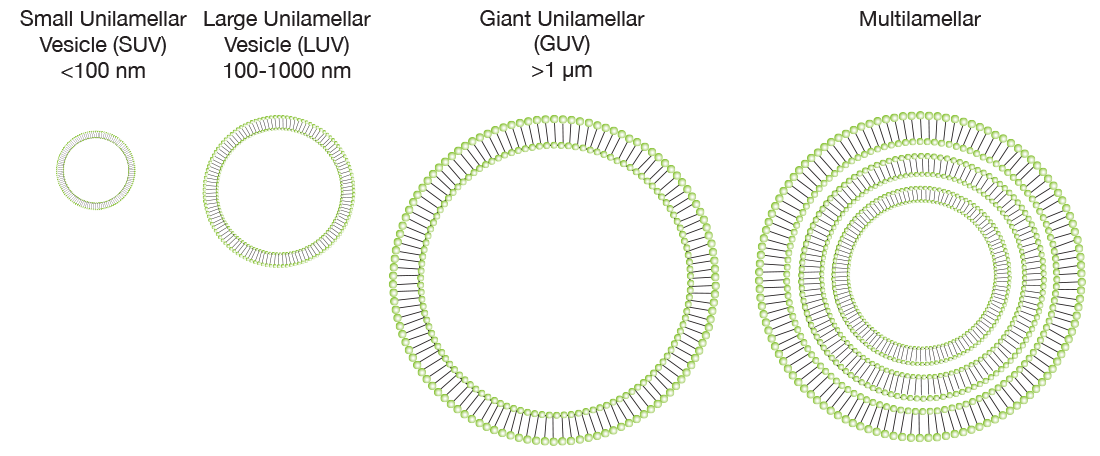
\includegraphics[width=0.8\textwidth]{img/guv}
  \vfill
  \raggedright
  Son agregados que no están en equilibrio termodinámico
\end{frame}

\begin{frame}{GUVs}
  \emph{Giant Unilamellar Vesicles}: \o 1--100 $\mu m$\\
  Una sola capa ($\approx 4 nm$) compuesta de moléculas \emph{anfifílicas}
  \vfill
  \centering
  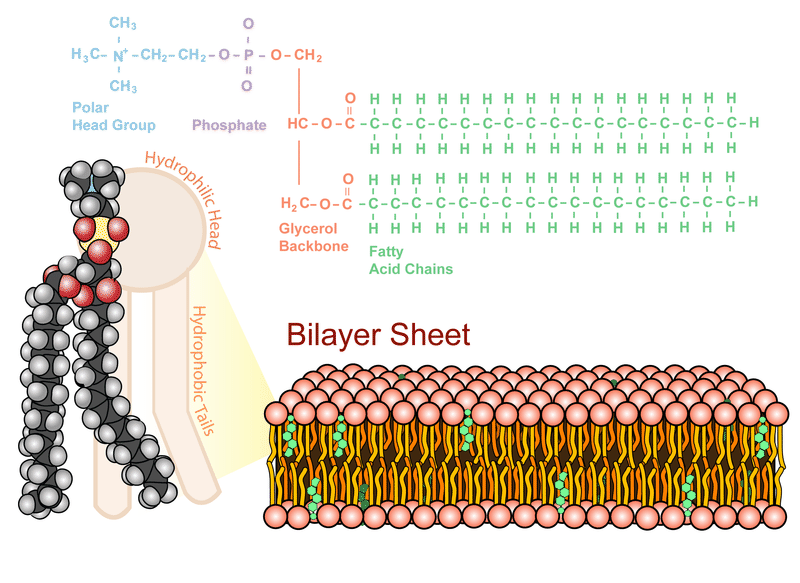
\includegraphics[width=0.6\textwidth]{img/bilayer}
\end{frame}

\section{Métodos de fabricación}

\begin{frame}{Hidratación}
  Hidratación controlada de films secos de lípidos depositados sobre una supercifie sólida
  \vfill
  \centering
  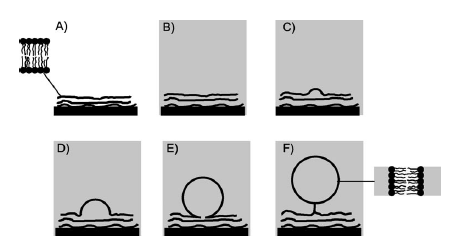
\includegraphics[width=6cm]{img/m_hydration}
  \vfill \small \raggedright 
  $\clubsuit$ \emph{Se obtiene un mayor control de la hidratación aplicando un campo eléctrico externo. Método más extendido en investigación.}
\end{frame}

\begin{frame}{Emulsión}
  GUVs formadas a partir de una emulsión agua/aceite:\\
    \hspace{1cm} A)  Estabilizada mediante lípidos\\
    \hspace{1cm} B)  Estabilizada mediante surfactantes\\
  \vfill
  \centering
  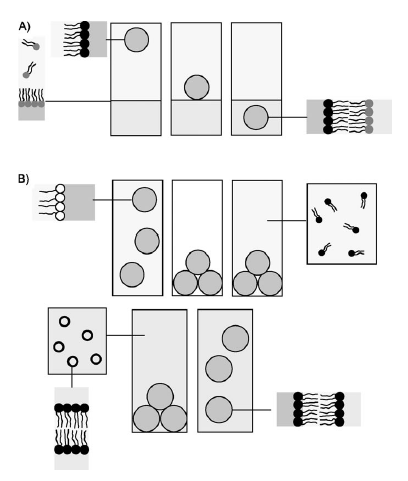
\includegraphics[width=4cm]{img/m_emulsion}
  \vfill \small \slshape \raggedright $\clubsuit$
  El tamaño de gota de agua de la emulsión marca el de las vesículas
\end{frame}

\begin{frame}{Doble emulsión}
  GUVs formadas a partir de una emulsión doble agua/aceite/agua\\
  \centering
  \vfill
  \centering
  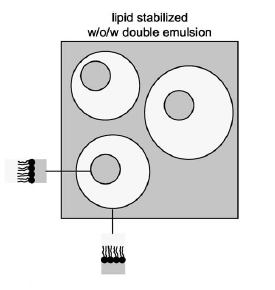
\includegraphics[scale=0.6]{img/m_doubleemulsion}
  \vfill \small \slshape \raggedright $\clubsuit$

\end{frame}

\begin{frame}{Fusión vesículas}
  Formación de GUVs a través de la fusión de vesículas de menor tamaño (SUVs y GUVs)
  \vfill
  \centering
  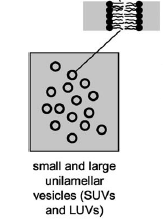
\includegraphics[scale=0.6]{img/m_suv}
\end{frame}

\begin{frame}{Bicapa plana}
  Formación de GUVs a partir de una bicapa lipídica plana
  \vfill
  \centering
  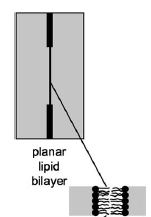
\includegraphics[scale=0.6]{img/m_planar}
\end{frame}

\begin{frame}{Lípidos disueltos}
  Formación de GUVs a partir de lípidos disueltos en un disolvente miscible con agua
  \vfill
  \centering
  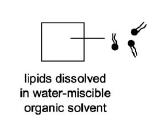
\includegraphics[scale=0.8]{img/m_lipids}
\end{frame}

\begin{frame}{Disolución micelar}
  Formación de GUVs a partir de una disolución micelar lipídica
  \vfill
  \centering
  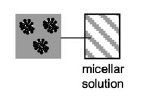
\includegraphics[scale=0.8]{img/m_micellar}
\end{frame}

\begin{frame}{Doble emulsión}
  Partiendo de un sistema bifásico agua/aceite, eliminar el aceite volátil de la doble emulsión agua/aceite/agua
  \vfill
  \centering
  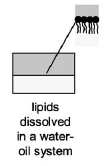
\includegraphics[scale=0.8]{img/m_lipidswo}
\end{frame}


\end{document}
